\documentclass{beamer} %%% FÜR VORTRAG MIT PAUSEN
%\documentclass[handout]{beamer}  %%% FÜR HANDOUT ALS PDF

\setbeamertemplate{navigation symbols}{}
\usetheme{Madrid}
\usecolortheme{seagull}
\beamersetuncovermixins{\opaqueness<1>{25}}{\opaqueness<2->{15}}
\usepackage[T1]{fontenc}
\usepackage{ae,aecompl}
\usepackage[ansinew]{inputenc}
\usepackage[ngerman]{babel}
\usepackage{amsmath}
\usepackage{amsfonts}
\usepackage[babel,german=quotes]{csquotes} %im deutschen übliche Anführungszeichen
\usepackage{verbatim}
\newcounter{saveenumi}
\newcommand{\seti}{\setcounter{saveenumi}{\value{enumi}}}
\newcommand{\conti}{\setcounter{enumi}{\value{saveenumi}}}
\usepackage{verbatim}

\begin{document}
\author[Willi Mutschler]{Willi Mutschler, M.Sc.}
\date{Summer 2014}
\institute[Institute of Econometrics]{Institute of Econometrics and Economic
Statistics\\University of M�nster\\willi.mutschler@uni-muenster.de}
\title{DSGE Methods}
\subtitle{Identification of DSGE models}

\begin{frame}
\titlepage
\end{frame}

\section{Identification}
\begin{frame}
\frametitle{\secname}
\begin{block}{Identification problem}
\begin{itemize}
\item Distinct parameter values do not lead to distinct probability distribution of data
   \item Source of identification influences findings
   \item Lack of identification leads to wrong conclusions from calibration and estimation
\end{itemize}
\end{block}
\begin{block}{Identification of DSGE models}
\begin{itemize}
\item concerned with two mappings
\begin{itemize}
  \item uniqueness of solution
      \begin{itemize}
          \item[$\hookrightarrow$] from the deep parameters to the reduced-form parameters
      \end{itemize}
  \item uniqueness of probability distribution
      \begin{itemize}
          \item[$\hookrightarrow$] from the solution to observable data
      \end{itemize}
    \end{itemize}
\item Bayesian approach
    \begin{itemize}
      \item circumvents badly shaped likelihood by using tight priors
      \item comparison of prior and posterior can be misleading
    \end{itemize}    
\end{itemize}
\end{block}
\end{frame}

\begin{frame}
\frametitle{\secname}
\begin{itemize}
    \item DSGE context: formal identification criteria via
    \begin{enumerate}[(i)]
      \item the autocovariogram (Iskrev 2010)
      \item the spectral density (Komunjer and Ng 2011 \& Qu and Tkachenko 2012)
      \item Bayesian indicators (Koop, Pesaran, and Smith 2012)
    \end{enumerate}
\end{itemize}
\end{frame}

\subsection{Basic Idea}
\begin{frame}
\frametitle{\secname}
Basic idea
\begin{itemize}
  \item Question of uniqueness of a solution, i.e. injectivity of functions
  \item Formally, given an objective function $\mathfrak{f}(\theta)$ a sufficient condition for $\theta_0$ being globally identified is given by
\begin{align*}
  \mathfrak{f}(\theta_1) =  \mathfrak{f}(\theta_0) \Rightarrow \theta_1 = \theta_0 \quad \text{for any }\theta_1 \in \Theta
\end{align*}
\item If this is only true in an open neighborhood of $\theta_0$, the identification of $\theta_0$ is local
   \item Population moments (mean, variance, autocovariance, spectrum) are functions of data
   \item[$\Rightarrow$] Check, whether mapping from $\theta$ to population moments is unique
   \item Conditions are in general only sufficient, unless data is generated from a Gaussian distribution (very common for DSGE)
\end{itemize}

\end{frame}


\begin{frame}
\footnotesize\frametitle{\secname}\framesubtitle{Approaches to time series analysis}
Time series analysis: try to explain regular behavior/patterns
  \begin{block}{Time domain approach}
    \begin{itemize}
      \item Idea: Regression of the present on the past
      \item Objective: Identify bunch of parameters
      \item Fundamental representation via autocovariances or Wold decomposition
    \end{itemize}
    \end{block}
\begin{block}{Frequency domain approach}
    \begin{itemize}
  \item Idea: Regression of the present on periodic sines and cosines, i.e. decomposition into regular components
  \item Regularity: periodic variations expressed as Fourier frequencies, driven by sines and cosines
  \item Objective: Identify dominant frequencies in a series
  \item Fundamental representation via spectral density
    \end{itemize}
  \end{block}
  \note{Frequency domain approach can set up the DGP for any time series\par}
  \note{Tendency of data to show periodic kinds of fluctuations.\par}
  \note{If two time series have the same Autocovariance, Wold decomposition or spectral density they are the same process.\par}
  \note{Examples: Detrending, deseasonalizing,etc. we implicitly assume that relations are different at different frequencies, one goal could be to isolate frequencies of interest\par}
  \note{Business Cycles vs. longer horizon, Money supply and nominal interest rates in short-run vs. long run\\}
  \note{Fourier analysis: well-behaved functions can be approximated over finite interval by a weighted combination of sine and cosine functions}
\end{frame}

\begin{frame}\frametitle{\secname}\framesubtitle{Approaches to time series analysis}
  \centering
  % Requires \usepackage{graphicx}
  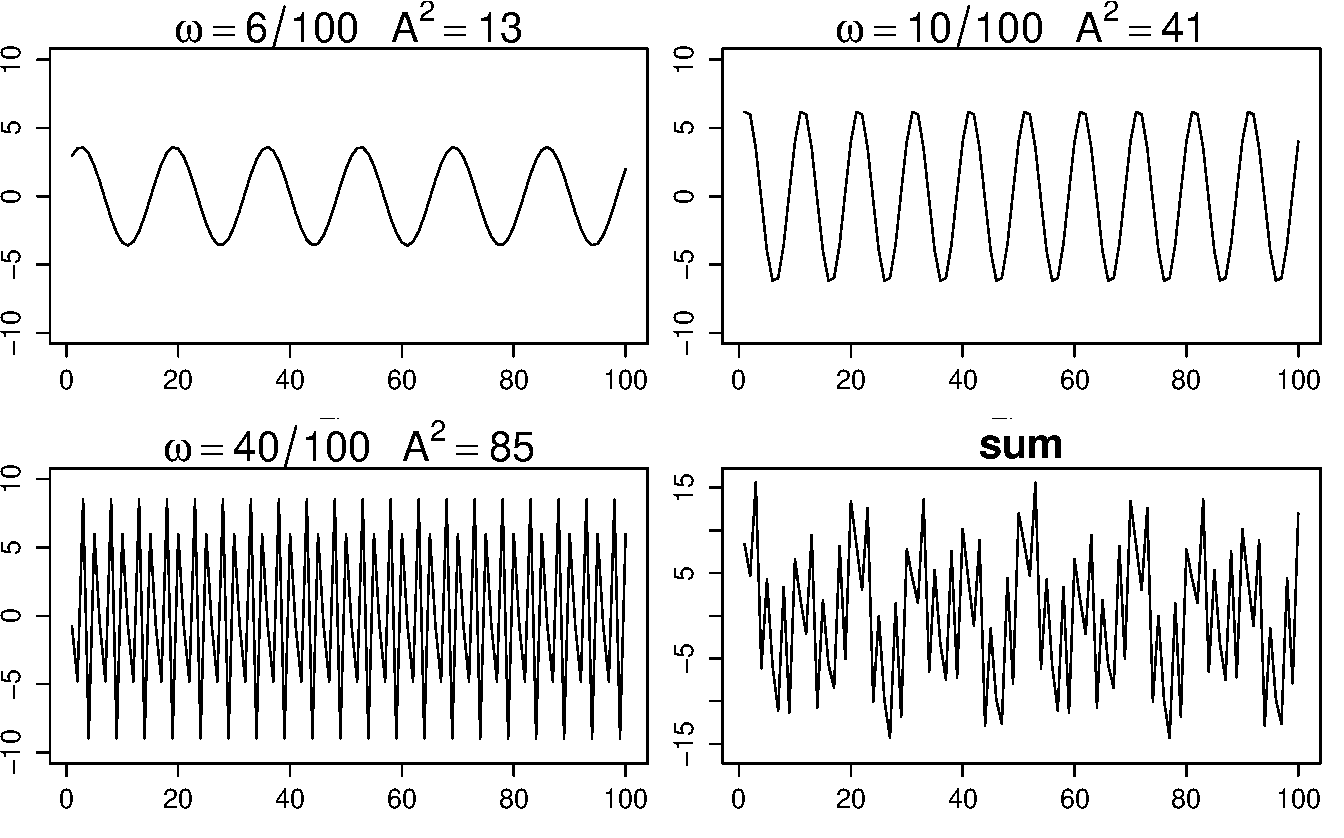
\includegraphics[width=\textwidth]{sines.pdf}
\end{frame}


\subsection{Iskrev's approach}
\begin{frame}\frametitle{Identification of DSGE-models}
\centering\Huge\subsecname
\end{frame}
\begin{frame}
\frametitle{\secname}\framesubtitle{\subsecname}
Iskrev (2010)'s approach:
\begin{itemize}
\item Idea: Check whether derivative of the mean and the predicted autocovariogram of observables w.r.t deep parameters has full rank\\ $\hookrightarrow$ Time domain approach
 \item Collect for $t=0,1,\dots,T-1$ all elements in a vector
\begin{align*}
m(\theta,T) &:= \begin{pmatrix}\mu_d' & vech(\Sigma_d)'& vec(\Sigma_d(1))'&\dots& vec(\Sigma_d(T-1))'\end{pmatrix}'
\end{align*}
\item If $m(\theta,q)$ is a continuously differentiable function of $\theta$, then $\theta_0$ is locally identifiable if the Jacobian
    \begin{align*}
M(q) := \frac{\partial m(\theta_0,q)}{\partial \theta'}
\end{align*}
has full column rank at $\theta_0$ for $q\leq T$, i.e. equal to $n_\theta$.
\end{itemize}
\end{frame}

\begin{frame}
\frametitle{\secname}\framesubtitle{\subsecname}
Iskrev (2010)'s necessary condition:
\begin{itemize}
  \item Stack all elements of the mean and the solution matrices that depend on $\theta$ into a vector $\tau$:
\begin{align*}
  \tau(\theta) := \begin{pmatrix}\mu_d'&vec(h_x)'&vec(g_x)'&vech(\eta_x \eta_x')'&vech(\eta_d \eta_d')'\end{pmatrix}'
\end{align*}
and consider the factorization
\begin{align*}
  M(q) &= \frac{\partial m(\theta,q)}{\partial \tau(\theta)'} \frac{\partial \tau(\theta)}{\partial \theta'}.
\end{align*}
\item $\theta_0$ is locally identifiable if the rank of $J := \frac{\partial \tau(\theta_0)}{\partial \theta'}$ at $\theta_0$ is equal to $n_\theta$.
\item This condition is, however, only necessary, because $\tau$ may be unidentifiable.
\end{itemize}
\end{frame}

\begin{frame}
\frametitle{\secname}\framesubtitle{\subsecname}
Implementation and interpretation:
\begin{itemize}
  \item Compute derivatives analytically or numerically
      \item If $\theta$ is identifiable, $M(q)$ and is likely to have full rank for $q$ much smaller than $T$
      \item Rank deficiency: Evaluating the nullspace one can pinpoint problematic parameters
\end{itemize}
\end{frame}


\subsection{Komunjer and Ng's approach}

\begin{frame}\frametitle{Identification of DSGE-models}
\centering\Huge\subsecname
\end{frame}

\begin{frame}
\frametitle{\secname}\framesubtitle{\subsecname}
\begin{itemize}
\item Based upon results from control theory for minimal systems (observable input and output sequences): 
\begin{itemize}
\item minimality and invertibility are enough to characterize observational equivalence of spectral densities
\end{itemize} 
   \item Consider minimal DSGE model, i.e. dynamics are entirely driven by the smallest possible dimension of the state vector (and shocks)
  \item Derive \textbf{restrictions} implied by \textbf{equivalent spectral densities} without computing any autocovariances or the spectral density 
  \item[$\hookrightarrow$] \emph{(Time and) Frequency domain approach}
 \end{itemize}
\end{frame}

\begin{frame}
\frametitle{\secname}\framesubtitle{\subsecname}
\begin{itemize}
  \item Consider minimal DSGE model
\begin{align*}
  x_{2,t} &= \overline{x}_2 + \widetilde{\mathcal{A}} (x_{2,t-1}-\overline{x}_2) + \widetilde{\mathcal{B}} \varepsilon_t,\\
  d_t &= \overline{d} + \widetilde{\mathcal{C}} (x_{2,t-1}-\overline{x}_2) + \widetilde{\mathcal{D}} \varepsilon_t.
\end{align*}
i.e. smallest possible dimension $n_{x_2}$ of the state vector such that dynamics are entirely driven by $x_{2,t}$ and $\varepsilon_t$.
 \begin{enumerate}
   \item[(i)] Controllability: For any initial state, it is always possible to design an input sequence that puts the system in the desired final state, i.e. the matrix $\begin{bmatrix}\widetilde{\mathcal{B}}&\widetilde{\mathcal{A}}\widetilde{\mathcal{B}}&\dots&\widetilde{\mathcal{A}}^{n_{x_2}-1}\widetilde{\mathcal{B}}\end{bmatrix}$ has full row rank,
   \item[(ii)] Observability: Given the evolution of the input it is always possible to reconstruct the initial state by observing the evolution of the output, i.e. the matrix $\begin{bmatrix}\widetilde{\mathcal{C}}'&\widetilde{\mathcal{A}}'\widetilde{\mathcal{C}}'&\dots&\widetilde{\mathcal{A}}^{n_{x_2}-1'}\widetilde{\mathcal{C}}'\end{bmatrix}'$ has full column rank.
 \end{enumerate}
 \end{itemize}
\end{frame}

\begin{frame}\frametitle{\secname}\framesubtitle{\subsecname}
\begin{itemize}
  \item Since $d_t$ is weakly stationary and $\varepsilon_t$ is either white noise or iid:
\begin{align*}
  d_t = \bar{d}+ \widetilde{\mathcal{D}}e_t + \sum_{j=1}^\infty \widetilde{\mathcal{C}} \widetilde{\mathcal{A}}^{j-1} \widetilde{\mathcal{B}} \varepsilon_{t-j} = \bar{d} + \widetilde{H}_e(L^{-1};\theta)\varepsilon_t,
\end{align*}
where L is the lag-operator. For $z\in \mathbb{C}$ the transfer function (z-transform) is
\begin{align*}
  \widetilde{H}_\varepsilon(z;\theta) := \widetilde{\mathcal{D}} + \sum_{j=1}^\infty \widetilde{\mathcal{C}} \widetilde{\mathcal{A}}^{j-1} \widetilde{\mathcal{B}} z^{-j} = \widetilde{\mathcal{D}} +\widetilde{\mathcal{C}} \left[I_{n_{x_2}} - \widetilde{\mathcal{A}} z \right]^{-1} \widetilde{\mathcal{B}}.
\end{align*}
\end{itemize}
\end{frame}

\begin{frame}
\frametitle{\secname}\framesubtitle{\subsecname}
\begin{itemize}
  \item Collect all hyperparameters of the state space solution into a vector $\Lambda(\theta):= \left(vec(\widetilde{\mathcal{A}})',vec(\widetilde{\mathcal{B}})',vec(\widetilde{\mathcal{C}})',vec(\widetilde{\mathcal{D}})',vech(\Sigma_\varepsilon)'\right)'$
  \item For all $z\in \mathbb{C}$ the spectral density matrix of $d_t$ is defined as
\scriptsize\begin{align*}
  \Omega_d(z;\theta)&:= \Sigma_d + \sum_{j=1}^\infty \Sigma_d(j)z^{-j} + \sum_{j=1}^\infty \Sigma_d(-j)z^{-j}
  = \widetilde{H}_\varepsilon(z;\theta) \Sigma_\varepsilon(\theta) \widetilde{H}_\varepsilon(z^{-1};\theta)'.
\end{align*}\normalsize
  \item Observational equivalence of $\theta_0$ and $\theta_1$ is equivalent to $\forall z \in \mathbb{C}:$
\scriptsize\begin{align*}
\widetilde{H}_\varepsilon(z;\Lambda(\theta_1))\cdot\Sigma_\varepsilon(\theta_1)\cdot \widetilde{H}_\varepsilon(z^{-1};\Lambda(\theta_1))' &= \widetilde{H}_\varepsilon(z;\Lambda(\theta_0)) \cdot \Sigma_\varepsilon(\theta_0) \cdot \widetilde{H}_\varepsilon(z^{-1};\Lambda(\theta_0))'
\end{align*}\normalsize
implies $\theta_0=\theta_1.$
\item Equivalent spectral densities arise if
\begin{enumerate}
\item[(i)] for given $\Sigma_\varepsilon(\theta)$, each transfer function $\widetilde{H}_\varepsilon(z;\Lambda(\theta))$ is potentially obtained from a multitude of quadruples $(\widetilde{\mathcal{A}},\widetilde{\mathcal{B}},\widetilde{\mathcal{C}},\widetilde{\mathcal{D}})$,
\item[(ii)] there are many pairs $\widetilde{H}_\varepsilon(z;\Lambda(\theta))$ and $\Sigma_\varepsilon(\theta)$ that jointly generate the same spectral density.
\end{enumerate}
\end{itemize}
\end{frame}

\begin{frame}
\frametitle{\secname}\framesubtitle{\subsecname}
\begin{itemize}
\item Komunjer and Ng (2011) show that this is equivalent to the existence of a $n_{x_2}\times n_{x_2}$ similarity transformation matrix $T$ and a $n_\varepsilon \times n_\varepsilon$ full column rank matrix $U=L_\varepsilon(\theta_0)VL_\varepsilon(\theta_1)^{-1}$ such that
\begin{align*}
  \widetilde{\mathcal{A}}(\theta_1)&=T \widetilde{\mathcal{A}}(\theta_0)T^{-1},& \widetilde{\mathcal{B}}(\theta_1) &=T \widetilde{\mathcal{B}}(\theta_0)U,& \widetilde{\mathcal{C}}(\theta_1) &= \widetilde{\mathcal{C}}(\theta_0)T^{-1}\\
  \widetilde{\mathcal{D}}(\theta_1)&= \widetilde{\mathcal{D}}(\theta_0) U,& \Sigma_\varepsilon(\theta_1) &= U^{-1} \Sigma_\varepsilon(\theta_0) U^{-1'},&
\end{align*}
with $L_\varepsilon$ being the Cholesky decomposition of $\Sigma_\varepsilon(\theta)=L_\varepsilon L_\varepsilon'$ and $V$ a constant matrix such that $VV'=I$\\
~\\~\\\centering $\Rightarrow$ \textbf{Now we have mappings}!
\end{itemize}
\end{frame}

\begin{frame}
\frametitle{\secname}\framesubtitle{\subsecname}
\begin{itemize}
\item Define a continuously differentiable mapping $\delta:\Theta\times \mathbb{R}^{n_{x_2}^2}\times \mathbb{R}^{n_\varepsilon^2} \rightarrow \mathbb{R}^{n_\Lambda}$ as
\begin{align*}
  \delta(\theta,T,U) := \begin{pmatrix}
    vec(T\widetilde{\mathcal{A}}(\theta)T^{-1})\\
    vec(T \widetilde{\mathcal{B}}(\theta)U)\\
    vec(\widetilde{\mathcal{C}}(\theta)T^{-1})\\
    vec(\widetilde{\mathcal{D}}(\theta_0) U)\\
    vech(U^{-1} \Sigma_\varepsilon(\theta_0) U^{-1'})
  \end{pmatrix}.
\end{align*}
\item $\theta$ is now locally identifiable from the spectral density (or equivalently autocovariances) of $d_t$ at a point $\theta_0$ if and only if $\delta^S(\theta,T,U)$ is locally injective at $(\theta_0,I_{n_{x_2}},I_{n_\varepsilon})$
\item Sufficient condition: matrix of partial derivatives of $\delta^S(\theta,T,U)$ has full column rank at $(\theta_0,I_{n_{x_2}},I_{n_\varepsilon})$
\end{itemize}
\end{frame}

\begin{frame}
\frametitle{\secname}\framesubtitle{\subsecname}
\footnotesize\begin{align*}
  \Delta(\theta_0) &:= \begin{pmatrix}
    \frac{\partial \delta(\theta_0,I_{n_{x_2}},I_{n_\varepsilon})}{\partial \theta'} &
    \frac{\partial \delta(\theta_0,I_{n_{x_2}},I_{n_\varepsilon})}{\partial vec(T)'} &
    \frac{\partial \delta(\theta_0,I_{n_{x_2}},I_{n_\varepsilon})}{\partial vec(U)'}
  \end{pmatrix}\\
  &=\begin{pmatrix}
    \frac{\partial vec(\widetilde{\mathcal{A}})}{\partial \theta'} & \widetilde{\mathcal{A}}'\otimes I_{n_{x_2}}-I_{n_{x_2}} \otimes \widetilde{\mathcal{A}} & 0_{n_{x_2}^2\times n_\varepsilon^2}\\
    \frac{\partial vec(\widetilde{\mathcal{}B})}{\partial \theta'} & \widetilde{\mathcal{B}}' \otimes I_{n_{x_2}} & I_{n_\varepsilon}\otimes \widetilde{\mathcal{B}}\\
    \frac{\partial vec(\widetilde{\mathcal{C}})}{\partial \theta'} &- I_{n_{x_2}}\otimes \widetilde{\mathcal{C}} & 0_{n_d n_{x_2}\times n_\varepsilon^2}\\
    \frac{\partial vec(\widetilde{\mathcal{D}})}{\partial \theta'} & 0_{n_d n_{x_2}\times n_{x_2}^2} & I_{n_\varepsilon} \otimes \widetilde{\mathcal{D}}\\
    \frac{\partial vech(\Sigma_e)}{\partial \theta'} & 0_{(n_\varepsilon(n_\varepsilon+1)/2)\times n_{x_2}^2} & -2 \Xi_{n_\varepsilon}[\Sigma_e \otimes I_{n_\varepsilon}]
    \end{pmatrix}\\
   & =: \begin{pmatrix}
      \quad\Delta_\Lambda(\theta_0) & \qquad&\Delta_T(\theta_0) &\qquad\quad\quad &\Delta_U(\theta_0)\qquad
    \end{pmatrix}
\end{align*}
\scriptsize with $\Xi_{n_\varepsilon}$ being the left-inverse of the $n_\varepsilon^2+n_\varepsilon(n_\varepsilon+1)/2$ duplication matrix $\mathcal{G}_{n_\varepsilon}$ for $vech(\Sigma_e)$
\begin{block}{Order and rank condition}
\begin{itemize}\footnotesize
    \item Order (necessary): $ n_\theta + n_{x_2}^2 + n_\varepsilon^2 \leq n_\Lambda^S := (n_{x_2} +n_d)(n_{x_2} + n_\varepsilon) + n_\varepsilon(n_\varepsilon+1)/2$
    \item Rank (necessary and sufficient): $rank(\Delta^s(\theta_0))= n_\theta + n_{x_2}^2 + n_\varepsilon^2$
  \end{itemize}
\end{block}
\end{frame}

\begin{frame}
\frametitle{\secname}\framesubtitle{\subsecname}
Implementation and interpretation
\begin{itemize}
  \item Analytical or numerical derivatives
  \item Derive minimal state vector: Check observability and controllability
  \item Remove the entries from all solution matrices and its derivatives corresponding to redundant state variables
\item Model diagnostics via other submatrices
  \item Nullspace can be used to pinpoint problematic parameters
\end{itemize}
\end{frame}


\subsection{Qu and Tkachenko's approach}
\begin{frame}\frametitle{Identification of DSGE-models}
\centering\Huge\subsecname
\end{frame}

\begin{frame}
\frametitle{\secname}\framesubtitle{\subsecname}
\begin{itemize}
\item Idea: Check whether derivative of the spectrum of observables w.r.t the deep parameters has full rank  $\hookrightarrow$ Frequency domain approach
\item Assume that $d_t$ is covariance-stationary:
\begin{align*}
 d_t = \bar{d} + \sum_{j=0}^\infty D g_x h_x^j \sigma \eta_x \varepsilon_{t-j} + \eta_d\varepsilon_t = \bar{d} + H_\varepsilon(L;\theta)\varepsilon_t
\end{align*}
with $H_\varepsilon(L;\theta)= D g_x \left(I_{n_x}-h_x L\right)^{-1} \sigma \eta_x + \eta_d$
\item  Using the Fourier transformation the spectral density matrix $\Omega_d$ is
\begin{align*}
  \Omega_d(\omega,\theta) &= \frac{1}{2\pi} H_\varepsilon(e^{-i\omega};\theta)\cdot \Sigma_\varepsilon(\theta)\cdot H_\varepsilon(e^{-i\omega};\theta)^*,\qquad \omega \in [-\pi;\pi],
\end{align*}
with $^*$ denoting the conjugate transpose of a complex valued matrix
\end{itemize}
\end{frame}

\begin{frame}
\frametitle{\secname}\framesubtitle{\subsecname}
\begin{itemize}
\item The test focuses on\scriptsize
\begin{align*}
  \underbrace{G(\theta_0)}_{n_\theta \times n_\theta} = \int_{-\pi}^\pi \left(\frac{\partial vec(\Omega_d(\omega;\theta_0))'}{\partial \theta'}\right)'\left(\frac{\partial vec(\Omega(\omega;\theta_0))'}{\partial \theta'}\right) d\omega
    + \frac{\partial \mu_d(\theta_0)'}{\partial \theta}\frac{\partial \mu_d(\theta_0)}{\partial \theta'}.
\end{align*}\normalsize
\item $\theta$ is locally identifiable at a point $\theta_0$ from the mean and spectrum of $d_t$ if and only if $G(\theta_0)$ is nonsingular, that is its rank is equal to $n_\theta$.
\end{itemize}
\end{frame}

\begin{frame}
\frametitle{\secname}\framesubtitle{\subsecname}
Implementation and interpretation
\begin{itemize}
  \item Derivative of $\Omega_d(\omega;\theta_0)$ can be calculated analytically or numerically, but numerically approximate integral
\item Full rank $G$ or $\overline{G}$: identification via spectrum or mean and spectrum
  \item Rank deficiency: check whether the diagonal elements of $G$ or $\overline{G}$ are nonzero
\end{itemize}
\end{frame}

\section{Exercise: Identification of An and Schorfheide (2007)}
\begin{frame}\frametitle{}
\begin{center}\Huge\secname\end{center}
\end{frame}

\begin{frame}
\frametitle{\secname}
Consider the An and Schorfheide (2007) model
\begin{enumerate}
\item Write a mod file for the log-linearized model.
\item Run and interpret Dynare's identification command.
\item Harder: Implement the other criteria based on ranks using numerical derivatives. Compare the results.
\end{enumerate}
\end{frame}

\section[Criteria Bayesian]{Bayesian identification criteria}
\begin{frame}\frametitle{}
\begin{center}\Huge\secname\end{center}
\end{frame}


\subsection{Koop, Pesaran, and Smith (2013)'s approach}
\begin{frame}
\frametitle{\secname}\framesubtitle{\subsecname}
Koop, Pesaran, and Smith (2013, JBES)'s approach
\begin{itemize}
  \item Indicates weak identification using Bayesian simulation techniques (Bayesian-learning-rate-indicator)
  \item Rate at which the posterior precision of a given parameter gets updated with the sample size T using simulated data
  \item For not identified or weakly identified parameters this rate is slower than T
\end{itemize}

\end{frame}


\begin{frame}\frametitle{\secname}\framesubtitle{\subsecname}
Implementation and interpretation
\begin{itemize}
\item Simulate data, divide into growing subsamples
\item Calculate variance or precision via
	\begin{itemize}
	\item Hessian (analytically or numerically) at posterior mode 
	\item MCMC variance of posterior distribution
	\end{itemize}
\item Precision divided by sample size will go to
	\begin{itemize}
	\item zero for weakly identified parameters
	\item a constant for identified parameters
	\end{itemize}
\end{itemize}
\end{frame}

\section{Comparison}
\begin{frame}\frametitle{}
\begin{center}\Huge\secname\end{center}
\end{frame}
\subsection{Identification criteria}
\begin{frame}
\frametitle{Comparison}\framesubtitle{}
\begin{itemize}
\item Methods differ due to different perspectives and assumptions:
\begin{itemize}
  \item Iskrev: time domain, very general assumptions (moments), compute derivative of autocovariogram
  \item Qu/Tkachenko: frequency domain, very general assumptions (VMA representation), compute derivative of spectrum
  \item Komunjer/Ng: (time and) frequency domain, strictest assumptions (minimality and left-invertibility), conditions without computing autocovariances or spectral density 
  \item KPS: Bayesian simulation approach
\end{itemize}
\item Computational issues and numerical errors
\begin{itemize}
  \item If feasible: Use analytical derivatives rather than numerical
  \item Isk: lag length, QT: subintervals for integral, KN: Find minimal representation, KPS: Filtering, Speed
  \item For all: numerical instability of solution algorithm, size of matrices
\end{itemize}
\item Methods include different model diagnostics
\end{itemize}
\end{frame}
\note{\begin{itemize}
  \item $J$ and $\Delta_\Lambda$ check mapping from structural parameters to reduced-form
  \item Rank deficient $\Delta_{\Lambda T}$ indicates that two structures (e.g. two different policies) might cause the same impulse response of the model given a known shock, however a rank-deficient $\Delta_{\Lambda U}$ includes also variation in the size of the shock.
  \item Qu and Tkachenko's test does not give such diagnostics, however, their approach can be used for a quasi maximum likelihood estimation in the frequency domain.
\end{itemize}
}

\end{document}

